\subsection{Model Setup} \label{ss:model_setup}
We used the MECCA box model for this study to determine the important chemical processes for ozone production under different temperatures and \ce{NO_x} conditions.
The MECCA box model was set up as described in \citet{Coates:2015} and updated to include vertical mixing with the free troposphere and a diurnal cycle for the PBL height based on the data from the BAERLIN 2014 campaign over Berlin, Germany \citep{Bonn:2016}. 
The supplementary material includes further details of these updates.

Simulations were performed to broadly simulate urban conditions of central Europe with equinoctical conditions.
The simulations started at 06:00 with a total run time of two days.
Methane was fixed at $1.7$~ppmv throughout the model run, carbon monoxide (CO) and ozone were initialised at $200$~ppbv and $40$~ppbv and then allowed to evolve freely throughout the the simulation.
All VOC emissions were held constant until noon of first day simulating a plume of freshly-emitted VOC.

In order to determine whether increased emissions of BVOC or faster chemistry is more important for the increase of ozone with temperature, model runs were repeated using a temperature-dependent and temperature-independent source of BVOC emissions. 
MEGAN2.1 \citep{Guenther:2012} specified the temperature-dependent BVOC emissions of isoprene, Sect.~\ref{ss:megan} provides further details. 
We considered isoprene as representative of all BVOC emissions as isoprene emissions are the most important on the global scale \citep{Guenther:2006}. 
In reality, many other BVOC are emitted from varying vegetation types \citep{Guenther:2006} and increased temperature can also increase AVOC emissions through increased evaporation \citep{Rubin:2006}.

\citet{Rasmussen:2013} indicated that changing the chemical mechanism used by a model may also change the simulated ozone-temperature relationship and warranted further investigation.
All simulations were repeated using different chemical mechanisms to investigate how well the relationship of ozone with temprature across \ce{NO_x} gradients is represented.
The reference chemical mechanism was the near-explicit Master Chemical Mechanism, MCMv3.2, \citep{Jenkin:1997}, \citep{Jenkin:2003}, \citep{Saunders:2003}, \citep{MCM_Site}.
The reduced chemical mechanisms in our study were Common Representative Intermediates, CRIv2 \citep{Jenkin:2008}, Model for ozone and related chemical tracers, MOZART-4 \citep{Emmons:2010}, Regional Acid Deposition Model, RADM2 \citep{Stockwell:1990} and the Carbon Bond Mechanism, CB05 \citep{Yarwood:2005}. 
\citet{Coates:2015} described these chemical mechanisms and the implementation of these chemical mechanisms in MECCA.
These reduced chemical mechanisms were chosen as they are commonly used by modelling groups in 3D regional and global models.

Separate box model simulations were performed with systematically varying the temperature between $288$ and $313$~K ($15$~--~$40$~\degree C). 
The only source of \ce{NO_x} emissions in the box model was a constant source of NO emissions. 
Box model runs were performed with the NO emissions systematically varied from $5.0~\times~10^9$ to $1.5~\times~10^{12}$~molecules~(NO)~cm$^{-2}$~s$^{-1}$ at each temperature used in this study. 

\subsection{VOC Emissions} \label{ss:VOC_emissions}
{%
    \renewcommand{\arraystretch}{1.1}%
    \begin{table}%
        \centering%
        \caption{Total AVOC emissions in 2011 in tonnes from each SNAP category assigned from TNO-MACC\_III emission inventory and temperature-independent biogenic VOC emissions in tonnes from Benelux region assigned from EMEP. The allocation of these emissions to MCMv3.2, CRIv2, CB05, MOZART-4 and RADM2 species is found in the supplementary material.}%
        \begin{tabular}{llllllll}
    \hline \hline
    & \textbf{SNAP1} & \textbf{SNAP2} & \textbf{SNAP34} & \textbf{SNAP5} & \textbf{SNAP6} & \textbf{SNAP71} \\
    \hline
    Belgium & $4494$ & $9034$ & $22152$ & $5549$ & $42809$ & $6592$ \\
    Netherlands & $9140$ & $12173$ & $29177$ & $8723$ & $53535$ & $16589$ \\
    Luxembourg & $121$ & $44$ & $0$ & $1372$ & $4482$ & $1740$ \\
    \hline
    Total & $13755$ & $21251$ & $51329$ & $15644$ & $100826$ & $24921$ \\
    \hline
    & \textbf{SNAP72} & \textbf{SNAP73} & \textbf{SNAP74} & \textbf{SNAP8} & \textbf{SNAP9} & \textbf{BVOC} \\
    \hline
    Belgium & $2446$ & $144$ & $210$ & $6449$ & $821$ & $6533$ \\
    Netherlands & $3230$ & $1283$ & $1793$ & $10067$ & $521$ & $1356$ \\
    Luxembourg & $1051$ & $6$ & $324$ & $643$ & $0$ & $2057$ \\
    \hline
    Total & $6727$ & $1433$ & $2327$ & $17159$ & $1342$ & $9946$ \\
    \hline \hline
\end{tabular}% 
%
        \label{t:emissions}%
    \end{table}%
}
Typical emissions of urban AVOC over central Europe were taken from TNO-MACC\_III emission inventory for the Benelux (Belgium, Netherlands and Luxembourg) region for the year 2011.
TNO-MACC\_III is the current version of the TNO-MACC\_II emission inventory created using the same methodology as \citet{Kuenen:2014} and based upon improvements to the existing emission inventory during AQMEII-2 \citep{Pouliot:2015}. 

Temperature-independent emissions of the biogenic VOC isoprene and monoterpenes were calculated as a fraction of the total AVOC emissions from each country in the Benelux region.
This data was obtained from the supplementary data available from the EMEP (European Monitoring and Evaluation Programme) model \citep{Simpson:2012}.
Temperature-dependent emissions of isoprene are detailed in Sect.~\ref{ss:megan}.

AVOC emissions were allocated to SNAP (Selected Nomenclature for Air Pollution) source categories.
Table~\ref{t:emissions} shows the tonnes of NMVOC emissions from each SNAP category and the temperature-independent BVOC emissions.
These categorised AVOC emissions were assigned to chemical species and groups based on the country specific profiles for Belgium, the Netherlands and Luxembourg provided by TNO.
Most individual chemical species are represented by the MCMv3.2, otherwise the individual contributions of a group of NMVOC were further split into individual components using the detailed speciation of \citet{Passant:2002}.
For example, `xylenes' are one of the component chemical groups to many SNAP categories but the MCMv3.2 treats xylenes as the individual isomers (m-, o-, p-xylene) and the individual contributions of the individual isomers to a SNAP category was provided by \citet{Passant:2002}.
This approach was also used in \citet{vonSchneidemesser:2015} to allocate AVOC emissions from different solvent sector speciations to MCMv3.2 species.

Again similarly to \citet{vonSchneidemesser:2015}, the NMVOC emissions were first assigned to chemcial species represented by the MCMv3.2 and then mapped to the mechanism species representing NMVOC emissions in each reduced chemical mechanism.
The NMVOC emissions in the reduced chemical mechanisms were weighted by the carbon numbers of the MCMv3.2 species and the emitted mechanism species. 
The supplementary data outlines the primary NMVOC and calculated emissions with each chemical mechanism.

\subsection{Temperature Dependent Isoprene Emissions} \label{ss:megan}
\begin{figure}[t]%
    \centering%
    \caption{The estimated isoprene emissions (molecules~isoprene~cm$^{-2}$~s$^{-1}$) at each temperature step used in the study. Isoprene emissions were estimated using the MEGAN2.1 algorithm \citep{Guenther:2012}.}
    \label{f:isoprene_emissions}%
    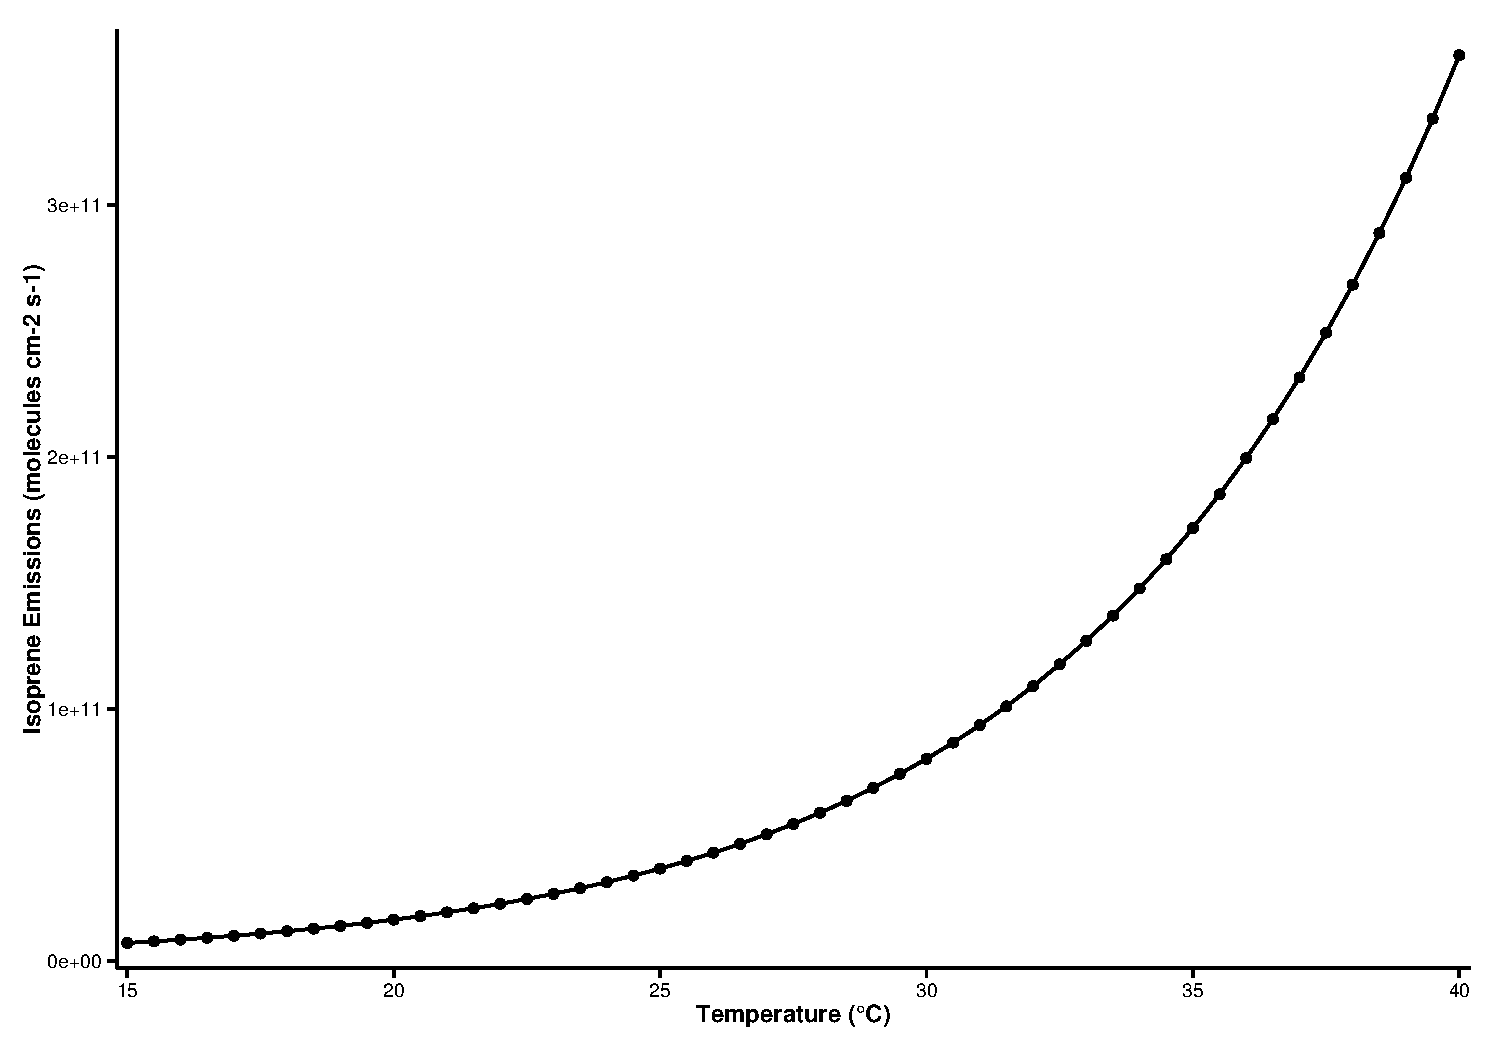
\includegraphics[width=\textwidth]{img/isoprene_emissions}
\end{figure}
Temperature-dependent emissions of isoprene were estimated using the MEGAN2.1 model for calculating the emissions of VOC from vegetation \citep{Guenther:2012}.
Emissions from plants are dependent on variables including temperature, radiation and age but for the purpose of our study we are only interested in the effects of temperature, hence all variables except temperature were held constant.

The MEGAN2.1 parameters were chosen to give similar isoprene mixing ratios at $20$~\degree C to the temperature-independent emissions of isoprene in order to compare the effects of increased isoprene emissions with temperature.
The estimated emissions of isoprene with MEGAN2.1 using these assumptions, are illustrated in Fig.~\ref{f:isoprene_emissions} and show the expected exponential increase in emissions with temperature \citep{Guenther:2006}.

We compared simulated isoprene mixing ratios from our simulations to measured isoprene emissions from the urban area of Essen, Germany \citep{Wagner:2014} to verify whether our chosen variables for MEGAN2.1 produced realistic isoprene mixing ratios.
At $20$~\degree C, the estimated emissions of isoprene lead to $0.07$~ppbv of isoprene in our model while at $30$~\degree C, the increased emissions of isoprene using MEGAN2.1 estimations lead to $0.35$~ppbv of isoprene in the model.
In the measurement campaign over Essen, $0.1$~ppbv of isoprene were measured at temperatures of $20$~\degree C and $0.3$~ppbv of isoprene were measured at $30$~\degree C.
This comparison indicates that the values chosen for calculating the temperature-dependent emissions of isoprene with MEGAN2.1 lead to reasonable values of isoprene mixing ratios.
